% Template LaTeX file for DAFx-08 papers
%
% To generate the correct references using BibTeX, run
%     latex, bibtex, latex, latex
% modified...
% - from DAFx-00 to DAFx-02 by Florian Keiler, 2002-07-08
% - from DAFx-02 to DAFx-03 by Gianpaolo Evangelista
% - from DAFx-05 to DAFx-06 by Vincent Verfaille, 2006-02-05
% - from DAFx-06 to DAFx-07 by Vincent Verfaille, 2007-01-05
%                          and Sylvain Marchand, 2007-01-31
% - from DAFx-07 to DAFx-08 by Henri Penttinen, 2007-12-12
%                          and Jyri Pakarinen 2008-01-28
%
% Template with hyper-references (links) active after conversion to pdf
% (with the distiller) or if compiled with pdflatex.
%
% 20060205: added package 'hypcap' to correct hyperlinks to figures and tables
%                      use of \papertitle and \paperauthorA, etc for same title in PDF and Metadata
%
% 1) Please compile using latex or pdflatex.
% 2) If using pdflatex, you need your figures in a file format other than eps! e.g. png or jpg is working
% 3) Please use "paperftitle" and "pdfauthor" definitions below


%%%%%%%%%%%%%%%%%%%%%%%%%%%%%%%%%%%%%%%%%%%%%%%%%%%%%%%%%%%%%%%%%%%%%
%%%%%%%%%%%%%%%%%%%%%%%%%%%%%%%%%%%%%%%%%%%%%%%%%%%%%%%%%%%%%%%%%%%%%
%%%%%%%%%%%%%%%%%%%%%%%%%%%%%%%%%%%%%%%%%%%%%%%%%%%%%%%%%%%%%%%%%%%%%
% 
% TTBlue Notes / Paper
% from conversation with Dave over coffee at Pre en Bulle in Albi
% 20 June 2008
% 
% 
% TTBlue is different from existing DSP libraries (such as Perry Cook's STK) in a number of ways:
% * Dynamic environment which itself can be queried for available components (using the TTFactory registry)
% * Dynamic binding, message passing architecture (reflective programming)
% 
% 
% Different from other C++ libraries in that it provides reflective programming techniques.
% Different from other languages with similar features in that it is implemented in C++ with good support for multiple platforms including embedded processor.
%  IEC 61508
%  Isograph
% 
% 
% Allows for:
% * programmatic creation of user interfaces
% * adaptive wrappers for various plug-in architectures (VST, AU, Max/MSP, SuperCollider)
% * dynamic, self-modifying networks of components 
% 
% 
% 
% 
% Try to see what we can learn from:
% * SuperCollider spawning thing for granular synthesis?
%  
% 
% 
% 
% Dynamic re-configuration of the signal networks and control structures means that TTBlue can be run on a web server and the signal chain defined (or re-defined) in real time on a web client using a GUI (such as a web browser or iPhone) or SMS.
% 
% One application of this is an installation or sculptural art work where you could tweak the behavior by sending it SMS messages using a phone.


% I would also like to develop a systematic approach for dealing with interpolation algorithms...
% Some sort of an interpolation library in TTBlue
% For example, this would allow us to apply the cubic interpolation everywhere without re-writing the code


%%%%%%%%%%%%%%%%%%%%%%%%%%%%%%%%%%%%%%%%%%%%%%%%%%%%%%%%%%%%%%%%%%%%%
%%%%%%%%%%%%%%%%%%%%%%%%%%%%%%%%%%%%%%%%%%%%%%%%%%%%%%%%%%%%%%%%%%%%%
%%%%%%%%%%%%%%%%%%%%%%%%%%%%%%%%%%%%%%%%%%%%%%%%%%%%%%%%%%%%%%%%%%%%%




%------------------------------------------------------------------------------------------
%  !  !  !  !  !  !  !  !  !  !  !  ! user defined variables  !  !  !  !  !  !  !  !  !  !  !  !  !  !
% Please use these commands to define title and author of the paper:
\def\papertitle{Templates for DAFx-08, Espoo, Finland}
\def\paperauthorA{The DAFx Crew and All Their Friends}
\def\paperauthorB{The Previous DAFx Crew}
\def\paperauthorC{Mary Goround}
\def\paperauthorD{The Lost Crew}


%------------------------------------------------------------------------------------------
\documentclass[twoside,a4paper]{article}
\usepackage{dafx_08}
\usepackage{amsmath,amssymb,amsfonts,amsthm}
\usepackage{subfigure,color}
\usepackage{euscript}
\usepackage[latin1]{inputenc}
\usepackage[T1]{fontenc}
\setcounter{page}{1}
\ninept

\usepackage{times}
% Saves a lot of ouptut space in PDF... after conversion with the distiller
% Delete if you cannot get PS fonts working on your system.

% pdf-tex settings: detect automatically if run by latex or pdflatex
\newif\ifpdf
\ifx\pdfoutput\relax
\else
   \ifcase\pdfoutput
      \pdffalse
   \else
      \pdftrue
\fi

\ifpdf % compiling with pdflatex
  \usepackage[pdftex,
    pdftitle={\papertitle},
    pdfauthor={\paperauthorA, \paperauthorB, \paperauthorC, \paperauthorD},
    colorlinks=false, % links are activated as colror boxes instead of color text
    bookmarksnumbered, % use section numbers with bookmarks
    pdfstartview=XYZ % start with zoom=100% instead of full screen; especially useful if working with a big screen :-)
  ]{hyperref}
  \pdfcompresslevel=9
  \usepackage[pdftex]{graphicx}
  \usepackage[figure,table]{hypcap}
\else % compiling with latex
  \usepackage[dvips]{epsfig,graphicx}
  \usepackage[dvips,
    colorlinks=false, % no color links
    bookmarksnumbered, % use section numbers with bookmarks
    pdfstartview=XYZ % start with zoom=100% instead of full screen
  ]{hyperref}
  % hyperrefs are active in the pdf file after conversion
  \usepackage[figure,table]{hypcap}
\fi

\title{\papertitle}

%-------------SINGLE-AUTHOR HEADER STARTS (uncomment below if your paper has a single author)-----------------------
%\affiliation{\paperauthorA}    % This command replaces \name{The DAFx Crew}
%{\href{http://www.acoustics.hut.fi/dafx08/}{Dept. of Signal Processing and Acoustics,} \\ Helsinki University of Technology, TKK \\ Espoo, Finland\\
%{\tt \href{mailto:dafx-08@acoustics.hut.fi}{dafx-08@acoustics.hut.fi}}}
%-----------------------------------SINGLE-AUTHOR HEADER ENDS------------------------------------------------------

%---------------TWO-AUTHOR HEADER STARTS (uncomment below if your paper has two authors)-----------------------
%\twoaffiliations{\paperauthorA, \sthanks{This work was supported by the XYZ Foundation}}
%{\href{
%http://www.acoustics.hut.fi/dafx08/}{Dept. of Signal Processing and Acoustics,} \\ Helsinki University of Technology, TKK \\ Espoo, Finland\\
%{\tt \href{mailto:dafx-08@acoustics.hut.fi}{dafx-08@acoustics.hut.fi}}
%}
%{\paperauthorB,\sthanks{This guy is a very good fellow}}
%{\href{http://www.acoustics.hut.fi/dafx08/}{Reading Group, Dept.~of Reading Sciences} \\ Univ.~of Universe, Sun \\ {\tt \href{mailto:dafx-08@acoustics.hut.fi}{dafx-08@acoustics.hut.fi}}
%}
%-------------------------------------TWO-AUTHOR HEADER ENDS------------------------------------------------------

%---------------THREE-AUTHOR HEADER STARTS (uncomment below if your paper has three authors)-----------------------
%\threeaffiliations{\paperauthorA, \sthanks{This work was supported by the XYZ Foundation}}
%{\href{
%http://www.acoustics.hut.fi/dafx08/}{Dept. of Signal Processing and Acoustics,} \\ Helsinki University of Technology, TKK \\ Espoo, Finland\\
%{\tt \href{mailto:dafx-08@acoustics.hut.fi}{dafx-08@acoustics.hut.fi}}
%}
%{\paperauthorB,\sthanks{This guy is a very good fellow}}
%{\href{http://www.acoustics.hut.fi/dafx08/}{Reading Group, Dept.~of Reading Sciences} \\ Univ.~of Universe, Sun \\ {\tt \href{mailto:dafx-08@acoustics.hut.fi}{dafx-08@acoustics.hut.fi}}
%}
%{\paperauthorC,\sthanks{She is a member of the Wheel Association}}
%{\href{http://www.acoustics.hut.fi/dafx08/}{Spinning Group, Dept.~of Turning Sciences} \\ Univ.~of Planets, Mars \\ {\tt \href{mailto:dafx-08@acoustics.hut.fi}{dafx-08@acoustics.hut.fi}}
%}
%-------------------------------------THREE-AUTHOR HEADER ENDS------------------------------------------------------

%----------------FOUR-AUTHOR HEADER STARTS (uncomment below if your paper has four authors)-----------------------
\fouraffiliations{
\paperauthorA, \sthanks{This work was supported by the XYZ Foundation}}
{\href{
http://www.acoustics.hut.fi/dafx08/}{Dept. of Signal Processing and Acoustics,} \\ Helsinki University of Technology, TKK \\ Espoo, Finland\\
{\tt \href{mailto:dafx-08@acoustics.hut.fi}{dafx-08@acoustics.hut.fi}}
}
{\paperauthorB,\sthanks{This guy is a very good fellow}}
{\href{http://www.acoustics.hut.fi/dafx08/}{Reading Group, Dept.~of Reading Sciences} \\ Univ.~of Universe, Sun \\ {\tt \href{mailto:dafx-08@acoustics.hut.fi}{dafx-08@acoustics.hut.fi}}
}
{\paperauthorC,\sthanks{She is a member of the Wheel Association}}
{\href{http://www.acoustics.hut.fi/dafx08/}{Spinning Group, Dept.~of Turning Sciences} \\ Univ.~of Planets, Mars \\ {\tt \href{mailto:dafx-08@acoustics.hut.fi}{dafx-08@acoustics.hut.fi}}
}
{\paperauthorD,\sthanks{Yes, senior}}
{\href{http://www.acoustics.hut.fi/dafx08/}{Unknown Group, Dept.~of Volatile Sciences} \\ Univ.~of Nowhere, Somewhere \\ {\tt \href{mailto:dafx-08@acoustics.hut.fi}{dafx-08@acoustics.hut.fi}}
}
%-------------------------------------FOUR-AUTHOR HEADER ENDS------------------------------------------------------

\begin{document}
% more pdf-tex settings:
\ifpdf % used graphic file format for pdflatex
  \DeclareGraphicsExtensions{.png,.jpg,.pdf}
\else  % used graphic file format for latex
  \DeclareGraphicsExtensions{.eps}
\fi

\maketitle

\begin{abstract}
This is the template file for the proceedings of the 11$^{\text{th}}$ International Conference on Digital Audio Effects (DAFx-08).
This template has been generated from WASPAA'99 templates and aims at producing conference proceedings in electronic form.
The format is essentially the one used for ICASSP conferences.
Please use either this \LaTeX{} or the accompanying Word formats when preparing your submission.
The templates are available in electronic form on the following website:
\\ \href{http://www.acoustics.hut.fi/dafx08/}{http://www.acoustics.hut.fi/dafx08/}. Thanks!

\end{abstract}

\section{Introduction}
\label{sec:intro}
This template can be found on the conference website.

\subsection{Figures}
\label{ssec:figures}
All figures should be centered on the column (or page, if the figure spans both columns).
Figure captions (in italic) should follow each figure and have the format given in Figure \ref{fft_plot}.
\begin{figure}[ht]
\centerline{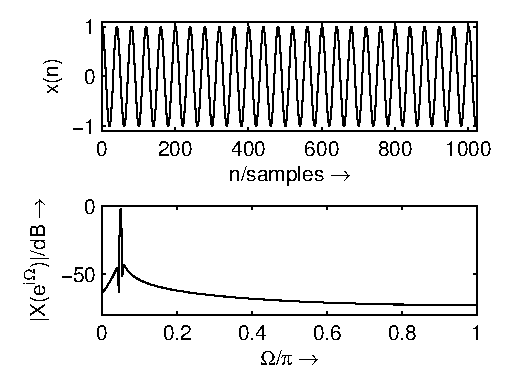
\includegraphics[scale=0.8]{fft_plot2}}
\caption{\label{fft_plot}{\it Sinusoid in time and frequency domain.}}
\end{figure}
Vectorial figures are preferred. For example when using
\texttt{Matlab}, export using either Postscript or PDF format. Also,
in order to provide a better readability, figure text font size
should be at list identical to footnote font size. To do so using
\texttt{Matlab}, use the \texttt{subplot} command before plotting.
If bitmap figures are used, please make sure that the resolution is
enough for print quality. Fig. \ref{ftt_plot2} illustrates an
example of a figure spanning two columns.
\begin{figure*}[ht]
\centerline{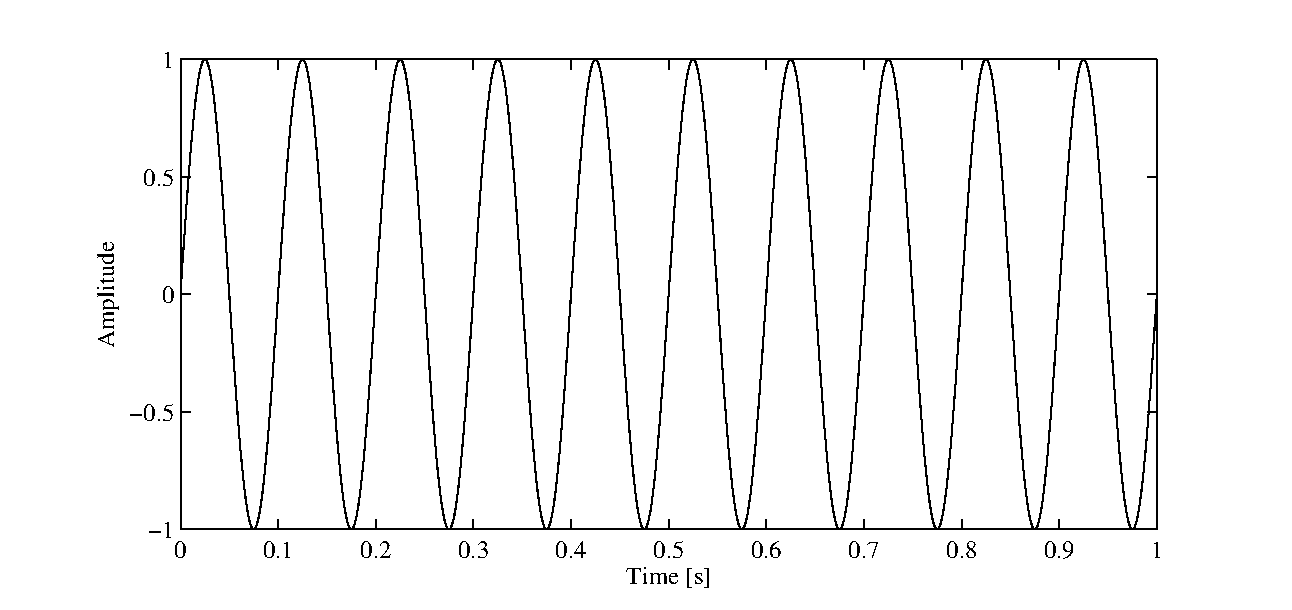
\includegraphics[width=5in,bb= 3 257 607 534]{TwoColumnSine2}} % The bounding box is set manually in this example. Useful for some .pdf figures.
\caption{\label{ftt_plot2}{\it A figure spanning two columns, as mentioned in Sec. \ref{ssec:figures}. }}
\end{figure*} % [width=5in,bb= 36 253 574 500]

\subsection{Tables}
As for figures, all tables should be centered on the column (or page, if the table spans both columns).
Table captions should be in italic, precede each table and have the format given in Table \ref{tab:example}.

\begin{table}[htdp]
  \caption{{\it Basic trigonometric values.}}
  \begin{center}
    \begin{tabular}{|c|c|}\hline
        angle ($\theta$, rad) & $\sin \theta$ \\\hline
    $\frac{\pi}{2}$ & 1 \\
    $\pi$ & 0 \\
    $\frac{3\pi}{2}$ & -1 \\
    $2\pi$ & 0 \\\hline
    \end{tabular}
  \end{center}
  \label{tab:example}
\end{table}

\begin{table*}[htdp]
  \caption{{\it Basic trigonometric values, spanning two columns.}}
  \begin{center}
    \begin{tabular}{|c|c|c|c|c|c|c|}\hline
        angle ($\theta$, rad) & $\sin \theta$ & $\cos \theta $ & $(\sin \theta)/2 $ & $(\cos \theta) /2 $ & $(\sin \theta)/3 $ & $(\cos \theta)/3$    \\\hline
    $\frac{\pi}{2}$ & 1 & 0 & 1/2 & 0 & 1/3 & 0 \\
    $\pi$ & 0 & -1 & 0 & -1/2 & 0 & -1/3\\
    $\frac{3\pi}{2}$ & -1 & 0 & -1/2 & 0 & -1/3 & 0 \\
    $2\pi$ & 0 & 1 & 0 & 1/2 & 0 & 1/3\\\hline
    \end{tabular}
  \end{center}
  \label{tab:example2}
\end{table*}

\subsection{Equations}
Equations should be placed on separate lines and numbered:

\begin{equation}
X(e^{j\Omega})=\sum_{n=0}^{N-1}x(n)e^{-j\Omega n}
\label{eq1}
\end{equation}
where the sequence $x(n)$ in equation (\ref{eq1}) is a windowed frame:
\begin{equation}
x(n)=s(n) w(n)
\label{eq2}
\end{equation}
with a window function $w(n)$.

\subsection{Page Numbers}
Page numbers will be added to the document electronically, so {\em please leave the numbering as is},
that is, the first page will start at page DAFX-1 and the last page, at most, will have to be DAFX-8
for the submission of papers for an oral presentation or DAFX-4 in the case of a poster presentation.

\subsection{References}
The references will be numbered in order of appearance \cite{Mitra:Kaiser:1993:DSP:handbook}, \cite{Haykin:1991:adaptive:filter}, \cite{Moorer:2000:AES:audio:millenium} and \cite{Nackaerts:2001:ICMC}. Please avoid listing references that do not appear in the text (we did the opposite in this template).

\subsubsection{Reference Format}
The reference format is the standard IEEE one. We recommend to use BibTeX to create the reference list.

\section{Conclusions}
This template can be found on the conference website.
For changing the number of author affiliations (1-4), uncomment the corresponding regions in the \texttt{DAFx08\_tmpl.tex} file.
Please, submit full-length papers (max.~8 pages for oral presentation and max.~4 pages for posters).
Submission is fully electronic and automated through the Conference Web Submission System.
DO NOT send us papers directly by e-mail.

\section{Acknowledgments}
Many thanks to the great number of anonymous reviewers!

%\newpage
\nocite{*}
\bibliographystyle{IEEEbib}
\bibliography{template} % requires file template.bib

\section{Appendix: Margin Check}
This section shows the column margins for the text. \bigskip\newline

Olihan Langholma isonen ja kielt\"{a}m\"{a}tt\"{a} pit\"{a}j\"{a}n p\"{a}\"{a}, eik\"{a} Alas-talo sit\"{a}
vastaan napissut, koska hyv\"{a}kin py\"{o}r\"{a} k\"{a}rrynrattaissa aina tarvitsee
akselinnavan huhkiaksensa kehill\"{a}ns\"{a}, ja koska tuolupuissakin tukki on
tarpeen, jotta on lointa ja loimissa t\"{a}mmi sukkulan sy\"{o}st\"{a} kuteitansa
ja kaiteen naputtaa kangastansa, mutta ylpe\"{a}ksi meni Alastalon niska
kuitenkin nyt ja tukan alla karahutteli veren varsa korskiansa, koska
viimein oltiin n\"{a}in pitk\"{a}ll\"{a}, ja vaelto nyt salissa k\"{a}\"{a}r\"{o} kourassa ja
kahden talven ty\"{o}n \"{a}hin\"{a} piirtopaperilla valmiina puhtain viivoin ja
linjaalivedoin, eik\"{a} Langholmallakaan muuta tekemist\"{a} kuin keikutella
keinutuolilla ja odotella niin kuin muutkin ja kuka hyv\"{a}ns\"{a}: napa kuin
napa, mutta rattaan hyrr\"{a} virstat j\"{a}tt\"{a}\"{a}; ja loimi tukilla lointa
tukilla, mutta kankaan verka vasta kyyn\"{a}riss\"{a} mitataan.

Olihan Langholma isonen ja kielt\"{a}m\"{a}tt\"{a} pit\"{a}j\"{a}n p\"{a}\"{a}, eik\"{a} Alas-talo sit\"{a}
vastaan napissut, koska hyv\"{a}kin py\"{o}r\"{a} k\"{a}rrynrattaissa aina tarvitsee
akselinnavan huhkiaksensa kehill\"{a}ns\"{a}, ja koska tuolupuissakin tukki on
tarpeen, jotta on lointa ja loimissa t\"{a}mmi sukkulan sy\"{o}st\"{a} kuteitansa
ja kaiteen naputtaa kangastansa, mutta ylpe\"{a}ksi meni Alastalon niska
kuitenkin nyt ja tukan alla karahutteli veren varsa korskiansa, koska
viimein oltiin n\"{a}in pitk\"{a}ll\"{a}, ja vaelto nyt salissa k\"{a}\"{a}r\"{o} kourassa ja
kahden talven ty\"{o}n \"{a}hin\"{a} piirtopaperilla valmiina puhtain viivoin ja
linjaalivedoin, eik\"{a} Langholmallakaan muuta tekemist\"{a} kuin keikutella
keinutuolilla ja odotella niin kuin muutkin ja kuka hyv\"{a}ns\"{a}: napa kuin
napa, mutta rattaan hyrr\"{a} virstat j\"{a}tt\"{a}\"{a}; ja loimi tukilla lointa
tukilla, mutta kankaan verka vasta kyyn\"{a}riss\"{a} mitataan.

Olihan Langholma isonen ja kielt\"{a}m\"{a}tt\"{a} pit\"{a}j\"{a}n p\"{a}\"{a}, eik\"{a} Alas-talo sit\"{a}
vastaan napissut, koska hyv\"{a}kin py\"{o}r\"{a} k\"{a}rrynrattaissa aina tarvitsee
akselinnavan huhkiaksensa kehill\"{a}ns\"{a}, ja koska tuolupuissakin tukki on
tarpeen, jotta on lointa ja loimissa t\"{a}mmi sukkulan sy\"{o}st\"{a} kuteitansa
ja kaiteen naputtaa kangastansa, mutta ylpe\"{a}ksi meni Alastalon niska
kuitenkin nyt ja tukan alla karahutteli veren varsa korskiansa, koska
viimein oltiin n\"{a}in pitk\"{a}ll\"{a}, ja vaelto nyt salissa k\"{a}\"{a}r\"{o} kourassa ja
kahden talven ty\"{o}n \"{a}hin\"{a} piirtopaperilla valmiina puhtain viivoin ja
linjaalivedoin, eik\"{a} Langholmallakaan muuta tekemist\"{a} kuin keikutella
keinutuolilla ja odotella niin kuin muutkin ja kuka hyv\"{a}ns\"{a}: napa kuin
napa, mutta rattaan hyrr\"{a} virstat j\"{a}tt\"{a}\"{a}; ja loimi tukilla lointa
tukilla, mutta kankaan verka vasta kyyn\"{a}riss\"{a} mitataan.

Olihan Langholma isonen ja kielt\"{a}m\"{a}tt\"{a} pit\"{a}j\"{a}n p\"{a}\"{a}, eik\"{a} Alas-talo sit\"{a}
vastaan napissut, koska hyv\"{a}kin py\"{o}r\"{a} k\"{a}rrynrattaissa aina tarvitsee
akselinnavan huhkiaksensa kehill\"{a}ns\"{a}, ja koska tuolupuissakin tukki on
tarpeen, jotta on lointa ja loimissa t\"{a}mmi sukkulan sy\"{o}st\"{a} kuteitansa
ja kaiteen naputtaa kangastansa, mutta ylpe\"{a}ksi meni Alastalon niska
kuitenkin nyt ja tukan alla karahutteli veren varsa korskiansa, koska
viimein oltiin n\"{a}in pitk\"{a}ll\"{a}, ja vaelto nyt salissa k\"{a}\"{a}r\"{o} kourassa ja
kahden talven ty\"{o}n \"{a}hin\"{a} piirtopaperilla valmiina puhtain viivoin ja
linjaalivedoin, eik\"{a} Langholmallakaan muuta tekemist\"{a} kuin keikutella
keinutuolilla ja odotella niin kuin muutkin ja kuka hyv\"{a}ns\"{a}: napa kuin
napa, mutta rattaan hyrr\"{a} virstat j\"{a}tt\"{a}\"{a}; ja loimi tukilla lointa
tukilla, mutta kankaan verka vasta kyyn\"{a}riss\"{a} mitataan.

Olihan Langholma isonen ja kielt\"{a}m\"{a}tt\"{a} pit\"{a}j\"{a}n p\"{a}\"{a}, eik\"{a} Alas-talo sit\"{a}
vastaan napissut, koska hyv\"{a}kin py\"{o}r\"{a} k\"{a}rrynrattaissa aina tarvitsee
akselinnavan huhkiaksensa kehill\"{a}ns\"{a}, ja koska tuolupuissakin tukki on
tarpeen, jotta on lointa ja loimissa t\"{a}mmi sukkulan sy\"{o}st\"{a} kuteitansa
ja kaiteen naputtaa kangastansa, mutta ylpe\"{a}ksi meni Alastalon niska
kuitenkin nyt ja tukan alla karahutteli veren varsa korskiansa, koska
viimein oltiin n\"{a}in pitk\"{a}ll\"{a}, ja vaelto nyt salissa k\"{a}\"{a}r\"{o} kourassa ja
kahden talven ty\"{o}n \"{a}hin\"{a} piirtopaperilla valmiina puhtain viivoin ja
linjaalivedoin, eik\"{a} Langholmallakaan muuta tekemist\"{a} kuin keikutella
keinutuolilla ja odotella niin kuin muutkin ja kuka hyv\"{a}ns\"{a}: napa kuin
napa, mutta rattaan hyrr\"{a} virstat j\"{a}tt\"{a}\"{a}; ja loimi tukilla lointa
tukilla, mutta kankaan verka vasta kyyn\"{a}riss\"{a} mitataan.

Olihan Langholma isonen ja kielt\"{a}m\"{a}tt\"{a} pit\"{a}j\"{a}n p\"{a}\"{a}, eik\"{a} Alas-talo sit\"{a}
vastaan napissut, koska hyv\"{a}kin py\"{o}r\"{a} k\"{a}rrynrattaissa aina tarvitsee
akselinnavan huhkiaksensa kehill\"{a}ns\"{a}, ja koska tuolupuissakin tukki on
tarpeen, jotta on lointa ja loimissa t\"{a}mmi sukkulan sy\"{o}st\"{a} kuteitansa
ja kaiteen naputtaa kangastansa, mutta ylpe\"{a}ksi meni Alastalon niska
kuitenkin nyt ja tukan alla karahutteli veren varsa korskiansa, koska
viimein oltiin n\"{a}in pitk\"{a}ll\"{a}, ja vaelto nyt salissa k\"{a}\"{a}r\"{o} kourassa ja
kahden talven ty\"{o}n \"{a}hin\"{a} piirtopaperilla valmiina puhtain viivoin ja
linjaalivedoin, eik\"{a} Langholmallakaan muuta tekemist\"{a} kuin keikutella
keinutuolilla ja odotella niin kuin muutkin ja kuka hyv\"{a}ns\"{a}: napa kuin
napa, mutta rattaan hyrr\"{a} virstat j\"{a}tt\"{a}\"{a}; ja loimi tukilla lointa
tukilla, mutta kankaan verka vasta kyyn\"{a}riss\"{a} mitataan.

Olihan Langholma isonen ja kielt\"{a}m\"{a}tt\"{a} pit\"{a}j\"{a}n p\"{a}\"{a}, eik\"{a} Alas-talo sit\"{a}
vastaan napissut, koska hyv\"{a}kin py\"{o}r\"{a} k\"{a}rrynrattaissa aina tarvitsee
akselinnavan huhkiaksensa kehill\"{a}ns\"{a}, ja koska tuolupuissakin tukki on
tarpeen, jotta on lointa ja loimissa t\"{a}mmi sukkulan sy\"{o}st\"{a} kuteitansa
ja kaiteen naputtaa kangastansa, mutta ylpe\"{a}ksi meni Alastalon niska
kuitenkin nyt ja tukan alla karahutteli veren varsa korskiansa, koska
viimein oltiin n\"{a}in pitk\"{a}ll\"{a}, ja vaelto nyt salissa k\"{a}\"{a}r\"{o} kourassa ja
kahden talven ty\"{o}n \"{a}hin\"{a} piirtopaperilla valmiina puhtain viivoin ja
linjaalivedoin, eik\"{a} Langholmallakaan muuta tekemist\"{a} kuin keikutella
keinutuolilla ja odotella niin kuin muutkin ja kuka hyv\"{a}ns\"{a}: napa kuin
napa, mutta rattaan hyrr\"{a} virstat j\"{a}tt\"{a}\"{a}; ja loimi tukilla lointa
tukilla, mutta kankaan verka vasta kyyn\"{a}riss\"{a} mitataan.



\end{document}
